\chapter{Theory Part}

\section{Question 1: Recovery Concepts}

\paragraph{1.} We assume that it is possible to write multiple pages
to stable storage atomically, and since we are forcing, we write all
changes to storage on commit. In this case everything ``just works'',
as long as no transactions is aborted after they have
committed. However this assumption does not necessarily hold in the
presence of cascading aborts. If we have cascading aborts, then we
need to able to undo the aborted, but forced commits -- and we need to
be able to do this even in the presence of a crash.

Alternatively we could decide that a transaction is never
\emph{really} committed, until it has no further possibilities for abort.

\paragraph{2.} Data stored in nonvolatile storage will survive a
crash, but the media itself can also fail. Datas stored on stable
storage can ``never'' be lost. In practice we do not only have stable
storage, but instead have probabilistic stable storage with a slightly
weaker guarantee: data stored will not be lost with probability larger
than $p$ (for some small value of $p$) -- unless your have bigger
problems to worry about such as survival.

\paragraph{3.} For the first part of the question, see
\autoref{fig:lolslides}. As for the second part:

\begin{itemize}
\item Assume we have a transaction, which alters a single page before
  aborting. The system crashes just as the transaction aborts. If we
  write the change to disc without forcing the log, then the system
  will not be able to undo the change on recovery, thus we do not have
  atomicity.
\item Assume we have a transaction, which alters a single page before
  committing successfully. The system crashes just after commit. If we
  have not written the log to disc, then we will not be able to live
  up to the promise of keeping the changes caused by the commit, thus
  we do not have durability.
\item This is enough for durability, since every transaction can be
  redone even in the event of a crash. The only situation where
  durability is broken is if we have cascading aborts.
\end{itemize}

\begin{figure}[H]
    \centering
    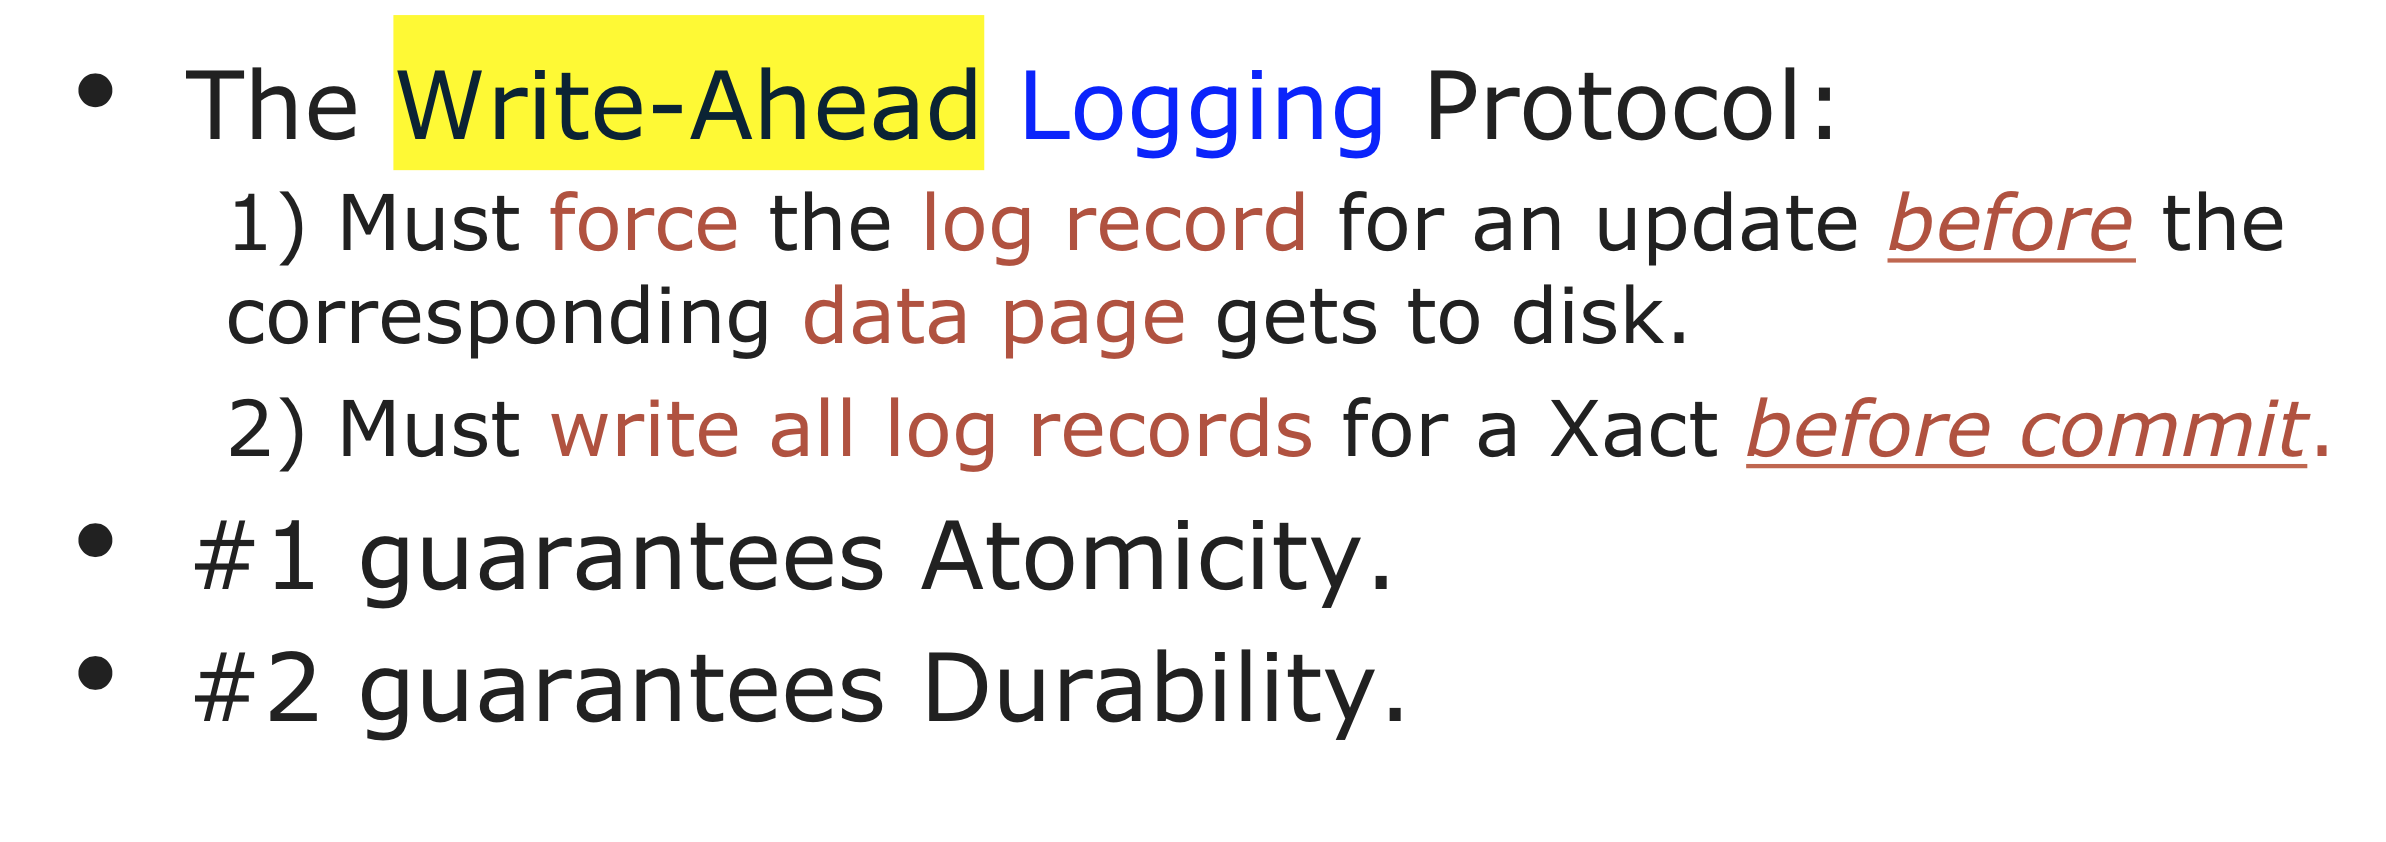
\includegraphics[width=\textwidth]{WAL-SS.png}
    \label{fig:lolslides}
    \caption{Forcing of log from the slides}
\end{figure}
